%%%%%%%%%%%%%%%%%%%%%%%%%%%%%%%%%%%%%%%%%%%%%%%%%%%%%%%%%%%%%%%%%%%%%%%%% 
% $Id$
% %%%%%%%%%%%%%%%%%%%%%%%%%%%%%%%%%%%%%%%%%%%%%%%%%%%%%%%%%%%%%%%%%%%%%%%%%
%
% Set de slides estudiando diferencias entre uso de Green3D o Green2D
% para problema cilindro infinito usando una seccion (rodaja 3D) del
% cilindro
%
% %%%%%%%%%%%%%%%%%%%%%%%%%%%%%%%%%%%%%%%%%%%%%%%%%%%%%%%%%%%%%%%%%%%%%%%%%

% %%%%%%%%%%%%%%%%%%%%%%%%%%%%%%%%%%%%%%%%%%%%%%%%%%%%%%%%%%%%%%%%%%%%%%%%%
\subsection{FEM Formulation}
% %%%%%%%%%%%%%%%%%%%%%%%%%%%%%%%%%%%%%%%%%%%%%%%%%%%%%%%%%%%%%%%%%%%%%%%%%

\begin{frame}[allowframebreaks]{Formulation}
  \begin{columns}
    \column{0.4\textwidth} \centering
    {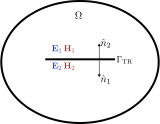
\includegraphics[angle=0,width=\textwidth]{scenario.pdf}}
    \column{0.6\textwidth}
    {
      \begin{align*}
        \hat{n}_1\times(\mu_r^{-1}&\nabla\times\vec{E}_1) - \frac{jk_0}{\eta}\vec{Y_{uu}}\hat{n}_1\times(\hat{n}_1\times\vec{E}_1) - \\
        - &\frac{jk_0}{\eta}\vec{Y_{ul}}\hat{n}_2\times(\hat{n}_2\times\vec{E}_2) = 0,
      \end{align*}
      \begin{align*}
        \hat{n}_2\times(\mu_r^{-1}&\nabla\times\vec{E}_2) - \frac{jk_0}{\eta}\vec{Y_{lu}}\hat{n}_1\times(\hat{n}_1\times\vec{E}_1) - \\
        - &\frac{jk_0}{\eta}\vec{Y_{ll}}\hat{n}_2\times(\hat{n}_2\times\vec{E}_2) = 0,
      \end{align*}

      \alert{Note that $\vec{Y}_{\rm xx}$ are relative to the vacuum admittance.}
    }
  \end{columns}

  \framebreak % %%%%%%%%%%%%%%%%%%%%%%%%%%%%%%%%%%%%%%

  Find $\vec{E} \in \vec{H}_0(\text{curl},\Omega)$ such that
  \begin{align*}
    &\Big(\nabla\times\vec{w},\mu_r^{-1}\nabla\times\vec{E} \Big)_\Omega - k_0^2\Big(\vec{w},\varepsilon_r\vec{E} \Big)_\Omega + 
    jk_0\Big\langle\hat{n}\times\vec{w},\hat{n}\times\vec{w}\Big\rangle_{\Gamma_{\text{C}}} = \\
    &\;\Big(\vec{w},\vec{F}\Big)_\Omega - 
    \Big\langle\hat{n}\times(\vec{w}\times\hat{n}),\vec{\Psi}_{\text{N}}\Big\rangle_{\Gamma_{\text{N}}} -
    \Big\langle\hat{n}\times(\vec{w}\times\hat{n}),\vec{\Psi}_{\text{C}}\Big\rangle_{\Gamma_{\text{C}}}
    \quad \forall \,\vec{w} \in \vec{H}_0(\text{curl},\Omega).
  \end{align*}
  
  with
  \begin{align}
    \Big(\vec{w},\vec{v}\Big)_\Omega &= \int_\Omega \vec{w}^* \cdot \vec{v} d\Omega, \nonumber\\
    \Big\langle \vec{w},\vec{v}\Big\rangle_{\Gamma} &= \int_\Gamma \vec{w}^* \cdot \vec{v} d\Gamma.\nonumber
  \end{align}
  
  \framebreak % %%%%%%%%%%%%%%%%%%%%%%%%%%%%%%%%%%%%%%
  For \emph{upper} elements on $\Gamma_{\rm TR}$ (sub-index u), we have
  \small
  \begin{align*}
    &{\rm LHS_u} \\
    &\; + j\frac{k_0}{\eta}\Big\langle\hat{n}\times(\vec{w}_u\times\hat{n}),\vec{Y_{uu}}\hat{n}\times(\vec{w}_u\times\hat{n})\Big\rangle_{\Gamma_{\text{TR}}} + j\frac{k_0}{\eta}\Big\langle\hat{n}\times(\vec{w}_u\times\hat{n}),\vec{Y_{ul}}\hat{n}\times(\vec{w}_l\times\hat{n})\Big\rangle_{\Gamma_{\text{TR}}} = \\
    &\;\;{\rm RHS_u},
  \end{align*}
  \normalfont
  whereas for \emph{lower} elements (sub-index l), we get
  \small
  \begin{align*}
    &{\rm LHS_l} \\
    &\; + j\frac{k_0}{\eta}\Big\langle\hat{n}\times(\vec{w}_l\times\hat{n}),\vec{Y_{lu}}\hat{n}\times(\vec{w}_u\times\hat{n})\Big\rangle_{\Gamma_{\text{TR}}} + j\frac{k_0}{\eta}\Big\langle\hat{n}\times(\vec{w}_l\times\hat{n}),\vec{Y_{ll}}\hat{n}\times(\vec{w}_l\times\hat{n})\Big\rangle_{\Gamma_{\text{TR}}} = \\
    &\;\;{\rm RHS_l},
  \end{align*}
  \normalfont
\end{frame}

\begin{frame}{DOFs implementation}
  \begin{itemize}
    \item The DOFs will be doubled for the faces and the interior edges.
    \item The exterior edges of $\Gamma_{\rm TR}$ are not doubled (unless they belong to a PBC).
  \end{itemize}
\end{frame}

% %%%%%%%%%%%%%%%%%%%%%%%%%%%%%%%%%%%%%%%%%%%%%%%%%%%%%%%%%%%%%%%%%%%%%%%%%
\subsection{Testing}
% %%%%%%%%%%%%%%%%%%%%%%%%%%%%%%%%%%%%%%%%%%%%%%%%%%%%%%%%%%%%%%%%%%%%%%%%%

\begin{frame}[allowframebreaks]{Problem to be solved}
  \begin{columns}
    \column{0.48\textwidth} \centering
    {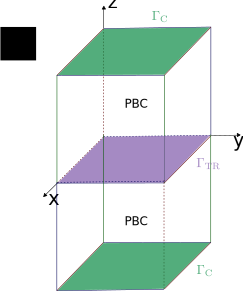
\includegraphics[angle=0,width=\textwidth]{tr_problem.pdf}}
    \column{0.48\textwidth}
    {
      Simulation of an infinite medium with transmission/reflection sheet that divides the space into two halves.
      \begin{itemize}
        \item $\Gamma_\text{TR}$: Transmission/reflection sheet defined with 
        \begin{equation*}
          \vec{Y} = \begin{bmatrix}
            \vec{Y}_{uu} & \vec{Y}_{ul} \\
            \vec{Y}_{lu} & \vec{Y}_{ll}
          \end{bmatrix}.
        \end{equation*}
        \item $\Gamma_\text{C}$: ABC with excitation with polarization $E_y$
        \item The vertical faces are set to PBC
      \end{itemize} 
    }
  \end{columns}
  \framebreak
  \includegraphics[angle=0,width=\textwidth]{tr_problem_gid.png}
\end{frame}

\begin{frame}{Testbench}
  \begin{itemize} 
    \item $\vec{Y} = \begin{bmatrix}
      0 & 0 \\
      0 & 0
    \end{bmatrix}$: sanity check, we should get same result as the first half with a PMC.
    \item $\vec{Y} = \mathbb{I}$: sanity check, we should get same result as the
    first half with an ABC and the other half with no field at all.
    \item Solve analytic problem with four media: final test.
    \begin{itemize}
      \item Obtain parameters for $\vec{Y}$ of the equivalent problem.
      \item Get same solutions for the electric field.
      \item Transparent? We will study approximation with higher values of admittance.
    \end{itemize}
  \end{itemize}
\end{frame}

% %%%%%%%%%%%%%%%%%%%%%%%%%%%%%%%%%%%%%%%%%%%%%%%%%%%%%%%%%%%%%%%%%%%%%%%%%
\subsection{HOFEM Implementation}
% %%%%%%%%%%%%%%%%%%%%%%%%%%%%%%%%%%%%%%%%%%%%%%%%%%%%%%%%%%%%%%%%%%%%%%%%%

\begin{frame}[allowframebreaks]{HOFEM implementation}
  \begin{itemize}
    \item New boundary condition: \texttt{TRBC}.
    \item New parameters in \texttt{boundary\_conditions\_module}
    \begin{itemize}
      \item \texttt{normal\_upper\_trbc}: $\hat{n}_{\rm TRBC}$. Upper side is the closer to $\hat{n}_{\rm TRBC}$.
      \item \texttt{admittance\_relative\_[3D,2D]\_tensor\_[,ll,ul,lu]}: relative values with respect to an admittance (as in AIBC).
      \item \texttt{neighbors\_trbc}: allocatable array of $2\times N_{\rm elem, TRBC}$ with:
      \begin{enumerate}
        \item $10\times$ upper element identifier + TRBC face.
        \item $10\times$ lower element identifier + TRBC face.
      \end{enumerate}
    \end{itemize}

    \framebreak

    \item Construction of \texttt{neighbors\_trbc} (only if TRBC are present):
    \begin{itemize}
      \item At \texttt{mesh\_interface\_constructor}.
      \item Using \texttt{surface\_set\_IDs}. They are given as consecutive (upper and then lower, or viceversa) elements. \alert{This is taken into account but it also looks for the element.}
      \item Possibility of different TRBCs.
      \item Identification of lower and upper elements.
      \item \alert{We need to detect here exterior edges (not done yet).}
    \end{itemize}
    \item Doubling unknowns (only if TRBC are present):
    \begin{itemize}
      \item At \texttt{mesh\_reordering\_module}.
      \item Using \texttt{neighbors\_trbc}.
      \item Modification of the DOFs for the lower elements.
    \end{itemize}   

    \framebreak

    \item Sparsity matrix assignments (only if TRBC are present):
    \begin{itemize}
      \item At \texttt{MUMPS\_set\_local\_JCN\_ICN\_RHS\_for\_matrix\_assembling}.
      \item Modification of the band number since we have \emph{coupled} elements.
      \item Non-symmetric matrix. \alert{If $\vec{Y}_{\rm lu} = \vec{Y}_{\rm ul}$, the matrix is symmetric (not yet detected).}
    \end{itemize}   
    \item Elementary terms (only if TRBC are present):
    \begin{itemize}
      \item Detect if lower or upper for identifying $\vec{Y}_{\rm uu}$, $\vec{Y}_{\rm ul}$, $\vec{Y}_{\rm lu}$, or $\vec{Y}_{\rm ll}$.
      \item Same term as AIBC for $\vec{Y}_{\rm uu}$ and $\vec{Y}_{\rm ll}$.
      \item Buffer for basis functions and Jacobian matrix for coupling terms $\vec{Y}_{\rm ul}$ and $\vec{Y}_{\rm lu}$.
    \end{itemize}
    \item FE assembly with \texttt{JCN} and \texttt{ICN}.
  \end{itemize}
\end{frame}
%%%%%%%%%%%%%%%%%%%%%%%%%%%%%%%%%%%%%%%%%%%%%%%%%%%%%%%%%%%%%%%%
